% !TeX root = funds.tex
\documentclass[paper.tex]{subfiles}
%\usepackage{pgfplots}

\begin{document}
	\section{Allocation of Funds}
	
	In order to determine the amount of money allocated to each school, we develop a model that follows utility theory. A utility study is appropriate for our model. Previously, we have determined a score for each university based on their qualifying characteristics. We would like to give more funding to a university with a higher score, thus, the utility of awarding a grant to a high-score school is also high. As scores decrease among universities, smaller and smaller awards will be distributed. We can model this change in award by modeling the utility for each school.
	\\
	
	First, we introduce some nomenclature.
	\begin{itemize}
		\item[($Q$)] The utility function
		\item[($S$)] The score given to each school based on aforementioned algorithms
		\item[($M_u$)] The amount of money awarded to a given school $u$ from the Goodgrant Foundation's pool
		\item[($P$)] Sum grant total (\$100,000,000)
	\end{itemize}
	There are several classes of utility functions that are commonly used in microeconomics. We will examine several utility functions in order to determine the function best fit for our situation. First let us consider a linear utility function.
	$$ Q(M_u) = SM_u $$
	
	\begin{center}
		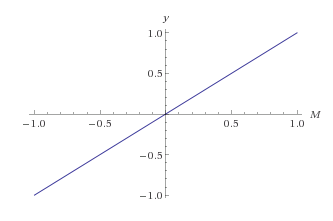
\includegraphics[width=0.5\linewidth]{images/UF1}
	\end{center}
	This function fits our model in some ways. The university with the largest amount of money will still receive the most grant money, but their allotment of money will be equivalent to $P$. This model assumes that the highest-scoring school will always be the best and only choice for award, and therefore the entire sum of grant money will go to the number one spot every time. This is, of course, not what we are looking for in a utility function. Let's try something a bit more complex.
	\\
	
	The second utility function falls under the category of isoelastic functions. Isoelastic functions return the same utility when scaled by an additive factor. \cite{norstad1999introduction}
	An important criterion for a successful isoelastic function is that the function has a negative second derivative, i.e. the function is concave down.  \[\frac{d^2a}{db^2} < 0\] 
	This means that our utility can be easily optimized within its boundary. A common isoelastic function is the natural logarithm. The natural logarithm meets the important criterion: \[\frac{d^2(\ln|b|)}{db^2} = \frac{-1}{b^2}\]  is less than one. However, a simple logarithm goes to negative $\infty$ at $0$, so we adjust by adding a factor of $1$ to the argument. Thus, our utility function for this model will be:
	$$ Q(M) = S(ln|M+1|) $$
\begin{center}
	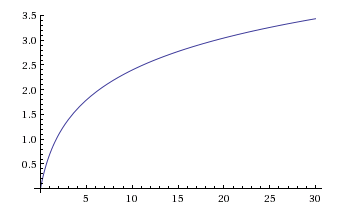
\includegraphics[width=0.5\linewidth]{images/UF2}
\end{center}
	
	We sum over all universities competing for grant money:
	$$ \sum_{U} Q(M_{u})  = \sum_{U} S_{U}(\ln|M_{u}+1|)  $$
	In order to award the largest sum of grant money to the school with the highest $S$ value, we optimize all $Q$ values by taking their derivatives with respect to all $M$ values.
	$$ \frac{d}{dM_{u}} \sum_{U}Q(M_{u})  = \sum_{u}\frac{S_{u}}{M_{u}} $$
	However, the derivative of the utility function with respect to $M$ and summed over all values of $M$ is simply the gradient of $Q$,
	$$ \frac{d}{dM_{u}} \sum_{U}Q(M_{u}) = \vec{\nabla} Q_{u}   $$
	and if we write our $S$ to $M$ ratio in vector form, we have:
	 
	$$ \vec{\nabla} Q_{u} =  \left( \begin{array}{c}
	\frac{S_{1}}{(M_{1}+1)} \\
	. \\
	.\\
	.\\
	\frac{S_{u}}{(M_{u}+1)}  \end{array} \right) $$
	\\
	
	We are attempting to solve for $M_{u}$ that we may give appropriate amounts of $P$ to each school with a high-enough score. We do not, however, have unlimited funds to allocate to these schools, so we need to generate a boundary parameter:
	$$ P = \sum_{u \in \UU} M_{u}   $$
	
	This way, the total amount given to all schools will not exceed the amount of money we are allowed to allocate. This is simple economics and budgeting, however, it mathematical implications allow us to solve for $M$. 
	\\\\
	Consider the method of Lagrange multipliers. Given the gradient of a vector field and a boundary condition for that field, Lagrange multipliers allow us to solve for the boundary function using a system of equations.
	
		$$\begin{cases}\vec{\nabla} Q_{u} = \lambda \vec{\nabla} M_{u}$$\\ $$\sum\limits_{u \in \UU} M_{u} - P = 0 \end{cases}$$ 
		
	The gradient of the sum of all vectors corresponding to grant awards ($M$) will be equal to $1$. This is because $M$ is a smooth, continuous function of one variable (itself).
	
	$$ \vec{\nabla} M_{u} = \vec{1} $$
	
	Implementing the above substitution and solving for $\lambda$, we can see that	
	$$\lambda = \dfrac{S_{u}}{M_{u}+1} $$
	
	So the money awarded to any given university $U$ is
	
	$$ \sum_{u \in \UU}M_{u} = \sum_{u \in \UU}(\dfrac{S_{u}}{\lambda} - 1) = P $$
	
	$$ \dfrac{1}{\lambda} \sum_{u \in \UU}(S_{u} + 1) = P $$
	
	$$ \lambda = \dfrac{1}{P + |\UU|}$$
	where $|U|$ is the total number of universities being considered for the grant, and $\sum_{u \in \UU}S_{u} = 1$ due to normalization of scores. Thus, the money given to each school becomes:
	
	$$ M_{Uu} = S_{u}(P+|\UU|) - 1$$
	
 	Still, this model is imperfect. It is important that we be allowed to give some universities exactly $0$ dollars, and the logarithmic function does not allow for $M$ values at $0$. Also, this utility function shows great appreciation for changes in $M$ near $0$, i.e. a change in grant award from $0$ to $\$1$ produces a large increase in utility. In reality, such an increase in utility would not occur near $M$ values of $0$, particularly for universities who deal with large sums of money all the time.
 	\\
 	We can adjust our utility function to account for these imperfections. Consider a the modified utility function $Q$:
 	
 	$$ Q(M_u) = S(ln|1+M_u^2| - 1) $$
 	
 	\begin{center}
 		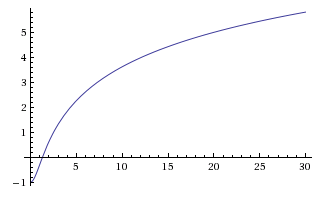
\includegraphics[width=0.5\linewidth]{images/UF3}
 	\end{center}
 	
 	This utility function is very similar to the first logarithmic function discussed. The function now has a value of nearly zero at zero. Points near the beginning of the graph are concave up, meaning that an increase in grant money will not impact the utility as greatly as it did in the previous model. The utility function can be solved for $M$ in the same fashion as before, producing:
 	
 	$$ M(S) = (P^2+1) \dfrac{\left(\sqrt{S^2 - \dfrac{(P - \sqrt{P^2S^2 + S^2 - 1})^2}{(P^2 + 1)^2}} -1\right)}{P - \sqrt{P^2S^2 + S^2 - 1}}$$
	
	Regardless, there are numerous utility functions that could be used in this particular situation. While most have a few imperfections, the logarithmic utility function serves our purpose well enough for the task at hand. The utility function's relationship to the size of grant awarded is nonetheless interesting.
\end{document}